\documentclass{book}
 
% \usepackage{ebook}
\usepackage{geometry}                % See geometry.pdf to learn the layout options. There are lots.
\geometry{letterpaper}                   % ... or a4paper or a5paper or ... 
%\geometry{landscape}                % Activate for for rotated page geometry
%\usepackage[parfill]{parskip}    % Activate to begin paragraphs with an empty line rather than an indent
\usepackage{graphicx}
\usepackage{sverb}
\usepackage{syntax}
\usepackage{framed}
\usepackage{array}
\usepackage{amsmath}
\usepackage{amsthm}
\usepackage{amsfonts}
\usepackage{proof}
%\usepackage{MnSymbol}
\usepackage{hyperref}
\usepackage{url}
\usepackage{xcolor}

% \pagecolor{black}
% \color{white}

%%%%%%%%%%%%%%%%%%%%%%%%%%%%%%%%%%%%%%%%%%%%%%%%%%%%%%%%%%%%%%%%%%%%%%%%%%
% Misc 
%%%%%%%%%%%%%%%%%%%%%%%%%%%%%%%%%%%%%%%%%%%%%%%%%%%%%%%%%%%%%%%%%%%%%%%%%%
\newcommand{\ie}{\emph{i.e.}}
\newcommand{\eg}{\emph{e.g.}}
\newcommand{\etc}{\emph{etc.}}

\newcommand{\comment}[1]{{\sf ({#1})}}

%%%%%%%%%%%%%%%%%%%%%%%%%%%%%%%%%%%%%%%%%%%%%%%%%%%%%%%%%%%%%%%%%%%%%%%%%%
% Environments 
%%%%%%%%%%%%%%%%%%%%%%%%%%%%%%%%%%%%%%%%%%%%%%%%%%%%%%%%%%%%%%%%%%%%%%%%%%

\newenvironment{normalenv}
{
  \renewcommand{\familydefault}{cmr}
  \normalfont
}
{
  \renewcommand{\familydefault}{cmss}
  \sffamily
}

%%%%%%%%%%%%%%%%%%%%%%%%%%%%%%%%%%%%%%%%%%%%%%%%%%%%%%%%%%%%%%%%%%%%%%%%%%
% Grammar 
%%%%%%%%%%%%%%%%%%%%%%%%%%%%%%%%%%%%%%%%%%%%%%%%%%%%%%%%%%%%%%%%%%%%%%%%%%

\makeatletter
\def\gr@implitem#1<#2> #3 {%
   \sbox\z@{\hskip\labelsep\grammarlabel{#2}{#3}}%
   \strut\@@par%
   \vskip-\parskip%
   \vskip-\baselineskip%
   \hrule\@height\z@\@depth\z@\relax%
   \item[\unhbox\z@]%
   \catcode`\<\active%
}
\makeatother

\newcommand{\keyw}[1]{\texttt{'}\textbf{#1}\texttt{'}}
\newcommand{\tkn}[1]{\texttt{#1}}

% -----------------------------------------------------------------------------
  %% doframeit draws a box around it argument by manipulating boxes.  It
  %% is used in the frame environments.
  %% 
  %%  Rene' Seindal (seindal@diku.dk) Fri Feb 12 16:03:07 1988
  %%  added \fboxrule and \fboxsep to \doframeit

\def\doframeit#1{\vbox{%
  \hrule height\fboxrule
    \hbox{%
      \vrule width\fboxrule \kern\fboxsep
      \vbox{\kern\fboxsep #1\kern\fboxsep }%
      \kern\fboxsep \vrule width\fboxrule }%
    \hrule height\fboxrule }}

  %% The frameit and Frameit environments formats text within a single 
  %% Anything can be framed, including verbatim text.

\def\frameit{\smallskip \advance \linewidth by -7.5pt \setbox0=\vbox \bgroup
\strut \ignorespaces }

\def\endframeit{\ifhmode \par \nointerlineskip \fi \egroup
\doframeit{\box0}}
% -----------------------------------------------------------------------------


\begin{document}
%\ebook

\title{Isolette Requirements \\
{\large (SAnToS Lab Version)}}

\author{
Adapted from DOT/FAA/AR-08/32\\
(DRAFT -- PLEASE DO NOT DISTRIBUTE)
}

\date{{\small \today}}

\maketitle

\tableofcontents

\pagestyle{plain}

\chapter{System Overview}
\label{chap:system-overview}

The system being specified is the Thermostat of an Isolette.\footnote{To simplify this example, the Operator Interface is treated as an external entity outside of the Thermostat.}  An Isolette is an incubator for an Infant that provides controlled temperature, humidity, and oxygen (if necessary). Isolettes are used extensively in Neonatal Intensive Care Units for the care of premature infants.

The purpose of the Isolette Thermostat is to maintain the air temperature of an Isolette within a desired range. It senses the Current Temperature of the Isolette and turns the Heat Source on and off to warm the air as needed. If the temperature falls too far below or rises too far above the Desired Temperature Range, it activates an alarm to alert the Nurse. The system allows the Nurse to set the Desired Temperature Range and to set the Alarm Temperature Range outside the Desired Temperature Range of which the alarm should be activated.

\section{System Content}
\label{sec:system-content}

The operational context of the Isolette Thermostat is shown in Figure~\ref{fig:state-concepts}.

%% import image
\begin{figure*}[ht]
  \centerline{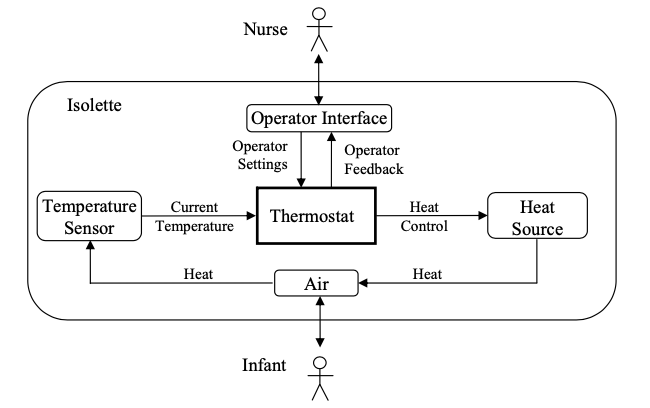
\includegraphics[width=\textwidth]{figures/thermostat-context-diagram.png}}
  \vspace{-.4cm}
  \caption{Context Diagram for the Isolette Thermostat}
  \vspace{-.4cm}
 \label{fig:state-concepts}
\end{figure*}


The Thermostat interacts directly with three entities that are part of the Isolette:
\begin{itemize}
\item The Temperature Sensor provides the Current Temperature of the air in the Isolette to the Thermostat.
\item The Heat Source heats the Air in the Isolette. It is turned on and off by the Heat Control.
\item The Operator Interface provides the Operator Settings for the Thermostat and receives Operator Feedback from the Thermostat.
\end{itemize}

The Thermostat also interacts indirectly with other entities outside of the Isolette:
\begin{itemize}
\item The Nurse who uses the Operator Interface to enter the Operator Settings and view the Operator Feedback.
\item The Air in the Isolette.
\item The Infant that is placed in the Isolette and is warmed by the Air.
\end{itemize}

\section{System Goals}
\label{sec:system-goals}

The high-level goals (G) of the system are:
\begin{itemize}
  \item G1—The Infant should be kept at a safe and comfortable temperature.
  \item G2—The Nurse should be warned if the Infant becomes too hot or too cold.
  \item G3—The cost of manufacturing the Thermostat should be as low as possible.
\end{itemize} 


\chapter{Operational Concepts}
\label{chap:operational-concepts}

The following use and exception cases describe how the operators
interact with the Isolette and the Thermostat. A summary of the use
and exception cases is provided in Table~\ref{tab:use-exception-cases}.
The actors and their primary goals are shown in Table~\ref{tab:actors-goals}.

\begin{table}
\begin{tabular}{|l|l|l|}
\hline   
{\bf ID} & \begin{minipage}[t]{2cm} {\bf Primary \\ Actor} \end{minipage} & {\bf Title and Description}
\\[1em]
\hline
~\ref{sec:uc-normal-operational} & Nurse & \emph{Normal Operation of Isolette:} \\
      &        & \hspace{3mm} 
                  \begin{minipage}[t]{11cm}
                    Describes the normal operation of the Isolette by the Nurse
                  \end{minipage}  
\\[1em]      
\hline
~\ref{sec:uc-configure} & Nurse & \emph{Configure the Isolette:} \\
      &        & \hspace{3mm} 
                  \begin{minipage}[t]{11cm}
                     Describes how the Nurse configures the Isolette and Thermostat for the Infant
                   \end{minipage}
\\[1em]
\hline
~\ref{sec:uc-maintain-temperature} & Thermostat & \emph{Maintain Desired Temperature:} \\
      &        & \hspace{3mm} 
                  \begin{minipage}[t]{11cm}
                     Describes how the Thermostat turns the Heat Source on and off to 
                     maintain the Current Temperature in the Isolette within the 
                     Desired Temperature Range
                   \end{minipage}
\\[1em]
\hline
~\ref{sec:ec-failure-maintain-safe-temperature} & Thermostat & \emph{Failure to Maintain Safe Temperature:} \\
      &            & \hspace{3mm} 
                     \begin{minipage}[t]{11cm}
                       Describes how the Thermostat and the Nurse respond when the 
                       Isolette is unable to maintain the Current Temperature 
                       within the Alarm Temperature Range
                     \end{minipage}
\\[1em]
\hline
~\ref{sec:ec-respond-failure} & Thermostat & \emph{Respond to Thermostat Failure:} \\
      &            & \hspace{3mm} 
                     \begin{minipage}[t]{11cm}
                        Describes how the Thermostat and the 
                        Nurse respond when the Thermostat detects an 
                        internal failure
                     \end{minipage}                                                         
\\[1em]
\hline
~\ref{sec:ec-failure-maintain-temperature} & Nurse & \emph{Failure to Maintain Desired Temperature:} \\
      &            & \hspace{3mm} 
                     \begin{minipage}[t]{11cm}
                        Describes how the Nurse deals with an Isolette that 
                        cannot keep the Current Temperature within the Desired 
                        Temperature Range but can keep the Current Temperature 
                        within the Alarm Temperature Range
                     \end{minipage}
\\
\hline                   
\end{tabular}   
\caption{Summary of Isolette Thermostat Use and Exception Cases}
\label{tab:use-exception-cases}
\end{table}

\begin{table}
\begin{tabular}{|l|l|}
\hline
{\bf Actor} & {\bf Primary Goals of the Actor} \\\hline
Nurse & \begin{minipage}[t]{11cm}
        Provide the Infant with proper nursing care, including keeping the Infant warm
        \end{minipage}
\\\hline
Infant & \begin{minipage}[t]{11cm}
         Be comfortable and healthy
         \end{minipage}
\\\hline
Isolette & \begin{minipage}[t]{11cm}
           Hold the Infant and maintain the Current Temperature within the Desired Temperature Range
           \end{minipage}
\\\hline
Thermostat & \begin{minipage}[t]{11cm}
             Maintain Current Temperature in the Isolette within the Desired Temperature Range
             \end{minipage}
\\\hline
\end{tabular}
\caption{Isolette Thermostat Primary Actors and Goals}
\label{tab:actors-goals}
\end{table}

\section{Use Case:  Normal Operation of Isolette}
\label{sec:uc-normal-operational}

This use case describes the normal operation of the Isolette by the Nurse.

\begin{itemize}
\item Related System Goals: G1 and G2
\item Primary Actor: Nurse
\item Precondition:
  \begin{itemize}
  \item Infant is ready to be placed in the Isolette
  \item Isolette and Thermostat are turned off
   \end{itemize}
\item Postcondition:
  \begin{itemize}   
  \item Infant is removed from the Isolette
  \item Isolette and Thermostat are turned off
  \end{itemize}
\item Main Success Scenario
  \begin{enumerate}
  \item Nurse turns on the Isolette
  \item Isolette turns on the Thermostat
  \item  Thermostat initializes and enters its normal mode of
    operation (exception case 1)
     (UC \ref{sec:ec-respond-failure}, Section~\ref{subsec:MRM-fun}, and Section~\ref{subsec:MMMF})
  \item Nurse configures the Isolette for the needs of the Infant (~\ref{sec:uc-configure})
  \item Nurse waits until the Current Temperature is within the Desired Temperature
            Range (~\ref{sec:ec-failure-maintain-temperature} and ~\ref{subsec:MRI-fun})
  \item Nurse places the Infant in the Isolette
  \item Isolette maintains Desired Temperature (~\ref{sec:uc-maintain-temperature})
  \item Nurse confirms that the Current Temperature is in the Desired Temperature Range during rounds (~\ref{sec:ec-failure-maintain-temperature} and ~\ref{subsec:MRI-fun})
  \item Nurse removes Infant
  \item Nurse turns off the Isolette
  \item Isolette turns off the Thermostat
  \end{enumerate}
\item Exception Case 1:
  \begin{enumerate}
  \item Alarm is activated because Current Temperature is outside the Alarm
Temperature Range (~\ref{subsec:manage-alarm-function})
  \item Nurse ignores the Alarm\footnote{In the interest of simplicity, the functionality to turn the Alarm off is not specified. As an exercise, the reader might want to consider what changes would be necessary to add this capability to the example.}
  \item Continue with Main Success Scenario, step 4.
  \end{enumerate}
\end{itemize}  

\section{Use Case:  Configure The Isolette}
\label{sec:uc-configure}

This use case describes how the Nurse configures the Isolette and Thermostat for the Infant.

\begin{itemize}
\item Related System Goals: G1 and G2
\item Primary Actor: Nurse
\item Precondition: The Isolette and Thermostat are turned on
\item Postcondition:
  \begin{itemize}
   \item The Desired Temperature Range is set for the needs of the Infant
   \item The Alarm Temperature Range is set for the needs of the Infant
   \item The Current Temperature in the Isolette is in the Desired Temperature Range
   \end{itemize}
\item Main Success Scenario:
   \begin{enumerate}
   \item Nurse sets the Alarm Temperature Range for the Infant (~\ref{subsec:MMIF})
   \item Nurse sets the Desired Temperature Range for the Infant (~\ref{subsec:MRI-fun})
   \item Thermostat maintains Desired Temperature Range (~\ref{sec:uc-maintain-temperature})
   \end{enumerate}
 \end{itemize}  

\section{Use Case: Maintain Desired Temperature}
\label{sec:uc-maintain-temperature}

This use case describes how the Thermostat turns the Heat Source on and off to maintain the
Current Temperature in the Isolette within the Desired Temperature Range.

\begin{itemize}
\item Related System Goals: G1
\item Primary Actor: Thermostat
\item Precondition: Isolette and Thermostat are turned on
\item Postcondition:
  \begin{itemize}
  \item Isolette and Thermostat are turned on
  \item Current Temperature is in the Desired Temperature Range
  \end{itemize}
\item Main Success Scenario:
  \begin{enumerate}
  \item Current Temperature falls below the Desired Temperature Range
  \item Thermostat turns the Heat Source on to warm up the Isolette (~\ref{subsec:manage-heat-source})
  \item Current Temperature rises above the Desired Temperature Range
  \item Thermostat turns the Heat Source off to cool the Isolette (~\ref{subsec:manage-heat-source})
  \item Repeat steps 1 through 4
  \end{enumerate}
\end{itemize}

\section{Exception Case: Failure To Maintain Safe Temperature}
\label{sec:ec-failure-maintain-safe-temperature}

This exception case describes how the Thermostat and Nurse respond when the Isolette is unable
to maintain Current Temperature within the Alarm Temperature Range.

\begin{itemize}
\item Related System Goals: G2
\item Primary Actor: Thermostat
\item Precondition:
  \begin{itemize}
  \item The Isolette and Thermostat are turned on
  \item The Current Temperature is within the Alarm Temperature Range
  \item The Alarm is off
  \end{itemize}
\item Postcondition:
  \begin{itemize}
  \item The Isolette and Thermostat are turned on
  \item The Current Temperature is within the Desired Temperature Range
  \item The Alarm is off
  \end{itemize}
\item Main Success Scenario:
  \begin{enumerate}
  \item Current Temperature falls below or rises above the Alarm Temperature Range
  \item Thermostat activates the Alarm (~\ref{subsec:manage-alarm-function})
  \item Nurse responds to the Alarm and sees that the Display Temperature is in the
        Alarm Temperature Range (~\ref{subsec:MRI-fun})
  \item Nurse removes Infant from the Isolette
  \item Nurse corrects the problem, e.g., closing an open door (alternate course 1)
  \item Nurse waits until the Display Temperature is within the Desired Temperature
        Range (~\ref{sec:ec-failure-maintain-temperature} and ~\ref{subsec:MRI-fun})
  \item Nurse places Infant back in the Isolette
  \end{enumerate}
\item Alternate Course 1:
  \begin{enumerate}
  \item Nurse is unable to correct the problem
  \item Nurse obtains another Isolette
  \item Nurse starts normal operation of the new Isolette (~\ref{sec:uc-normal-operational})
  \end{enumerate}
\end{itemize}

\section{Exception Case: Respond To Thermostat Failure}
\label{sec:ec-respond-failure}

This exception case describes how the Thermostat and the Nurse respond when the Thermostat
detects an internal failure.

\begin{itemize}
\item Related System Goals: G2
\item Primary Actor: Thermostat
\item Precondition:
  \begin{itemize}
  \item The Isolette and Thermostat are turned on
  \item The Thermostat status is on
  \item The Alarm is off
  \end{itemize}
\item Postcondition:
  \begin{itemize}
  \item The Isolette and Thermostat are turned on
  \item The Current Temperature is in the Desired Temperature Range
  \item The Alarm is off
  \end{itemize}
\item Main Success Scenario:
  \begin{enumerate}
  \item Thermostat detects an internal failure (~\ref{subsec:detect-regulator-failure} and ~\ref{subsec:DMFF})
  \item Thermostat enters the FAILED mode (~\ref{subsec:MRM-fun} and ~\ref{subsec:MMMF})
  \item Thermostat sets its Displayed Status to failed (~\ref{subsec:MRI-fun} and ~\ref{subsec:MMIF})
  \item Thermostat activates the Alarm
  \item Nurse responds to the Alarm and sees that the Thermostat is failed
  \item Nurse removes Infant from the Isolette
  \item Nurse obtains another Isolette
  \item Nurse starts normal operation of the new Isolette (~\ref{sec:uc-normal-operational})
  \end{enumerate}
\end{itemize}

\section{Exception Case: Failure To Maintain Desired Temperature}
\label{sec:ec-failure-maintain-temperature}

This exception case describes how the Nurse handles an Isolette that cannot keep the Current
Temperature within the Desired Temperature Range, but can keep the Current Temperature
within the Alarm Temperature Range.

\begin{itemize}
\item Related System Goals: G1
\item Primary Actor: Nurse
\item Precondition:
  \begin{itemize}
  \item The Isolette and Thermostat are turned on
  \item The Current Temperature is not within the Desired Temperature Range
  \item The Current Temperature is within the Alarm Temperature Range
  \end{itemize}
\item Postcondition:
  \begin{itemize}
  \item The Isolette and Thermostat are turned on
  \item The Current Temperature is in the Desired Temperature Range
  \end{itemize}
\item Main Success Scenario:
  \begin{enumerate}
  \item Nurse attempts to correct the problem, e.g., closing an open door
  \item Nurse waits until the Current Temperature of the Isolette is within the Desired
        Temperature Range (alternate course 1) (~\ref{subsec:MRI-fun})
  \item Return to calling scenario
  \end{enumerate}
\item Alternate Course 1:
  \begin{enumerate}
  \item Display Temperature fails to enter the Desired Temperature Range (~\ref{subsec:MRI-fun})
  \item Nurse removes Infant from the Isolette
  \item Nurse obtains another Isolette
  \item Nurse starts normal operation of the new Isolette (~\ref{sec:uc-normal-operational})
  \item Return to calling scenario
  \end{enumerate}
\end{itemize}
\chapter{External Entities}
\label{chap:external-entities}

The following sections describe the external entities with which the Thermostat directly
interacts: the Temperature Sensor, the Operator Interface, and the Heat Source. The monitored
and controlled variables associated with each entity are listed, along with any environmental
assumptions made about the entity. An Isolette external entity is also defined to specify
environmental assumptions that span more than one external entity.

\section{Isolette}
\label{sec:isolette}

An Isolette is an incubator for an Infant that provides controlled temperature, humidity, and
oxygen (if necessary). It encompasses the Thermostat, the Temperature Sensor, the Operator
Interface, and the Heat Source. The following environmental assumptions are made by the
Thermostat about the Isolette

\begin{itemize}
\item EA-IS-1: When the Heat Source is turned on and the Isolette is properly shut, the
      Current Temperature will increase at a rate of no more than 1°F per minute.

      Rationale: If the Current Temperature can increase at a rate of more than 1°F per minute,
      the Thermostat may not be able to turn the Heat Source off quickly enough to maintain
      the Desired Temperature Range unless the allowed latency specified for the Heat Control
      is reduced.
\item EA-IS-2: When the Heat Source is turned off and the Isolette is properly shut, the
      Current Temperature will decrease at a rate of no more than 1°F per minute.

      Rationale: If the Current Temperature can decrease at a rate of more than 1°F per
      minute, the Thermostat may not be able to turn the Heat Source on quickly enough to
      maintain the Desired Temperature Range unless the allowed latency specified for the
      Heat Control is reduced.
\end{itemize}

\section{Temperature Sensor}
\label{sec:temperature-sensor}

The Temperature Sensor provides the Current Temperature of the Air in the Isolette to the
Thermostat. The monitored variables are shown in table ~\ref{tab:temp-sensor}.

\begin{table}
\begin{tabular}{|l|l|l|l|l|}
\hline
Name & Type & Range & Units & Physical Interpretation \\\hline
Current Temperature & Real & [68.0..105.0] & °F & Current air temperature inside Isolette \\\cline{2-4}
     & Current & \textbullet Invalid, Valid &  &  \\\hline
\end{tabular}
\caption{Thermostat Monitored Variables for Temperature Sensor}
\label{tab:temp-sensor}
\end{table}

\begin{itemize}
\item Table ~\ref{tab:temp-sensor} denotes initial value
\end{itemize}

The following environmental assumptions are made:

\begin{itemize}
\item EA-TS-1: The Current Temperature will be provided to the Thermostat in degrees
      Fahrenheit

      Rationale: Consistency with environmental-assumption Operator Interface EA-OI-1
\item EA-TS-2: The Current Temperature will be sensed to an accuracy of ±0.1°F.

      Rationale: An accuracy of 0.1°F is necessary to ensure the Thermostat can turn the Heat
      Source on and off quickly enough to maintain the Desired Temperature Range.
\item EA-TS-3: The Current Temperature will cover the range of at least 68.0° to 105.0°F.

      Rationale: This is the specified range of operation of the Isolette. The lower end of this
      range is useful for monitoring an Isolette that is warming to the Desired Temperature
      Range. The upper end is greater than the Upper Alarm Temperature to ensure that the
      Current Temperature will be sensed across the entire Alarm Temperature Range.
\end{itemize}

\section{Heat Source}
\label{sec:heat-source}

The Heat Source heats the Air in the Isolette. It is turned on and off by changing the value of the
Heat Control controlled variable. The controlled variables are shown in table ~\ref{tab:heat-source-variables}. No
environmental assumptions are made.

\begin{table}
\begin{tabular}{|l|l|l|l|l|}
\hline
Name & Type & Range & Units & Physical Interpretation \\\hline
Heat Control & Enumerated & Off, On &  & Command to turn Heat Source on and off \\\hline
\end{tabular}
\caption{Thermostat Controlled Variables for Heat Source}
\label{tab:heat-source-variables}
\end{table}

\section{Operator Interface}
\label{sec:operator-interface}

The Operator Interface provides the Operator Settings for the Thermostat and receives Operator
Feedback from the Thermostat. The environmental assumptions associated with the Operator
Interface are quite strong, which simplifies the manage Operator Interface Function. If these
assumptions were not satisfied by the Operator Interface external entity, the Manage Operator
Interface Function would need to be strengthened to ensure consistent inputs to the Thermostat.
The monitored and controlled variables are shown in tables ~\ref{tab:operator-interface-variables} and ~\ref{tab:oi-controlled-variables}, respectively.

\begin{table}
\begin{tabular}{|l|l|l|l|l|}
\hline
Name & Type & Range & Units & Physical Interpretation \\\hline
Operator Settings &  &  &  & Thermostat settings provided by operator \\\hline
\multicolumn{4}{|l|}{Desired Temperature Range} & Desired range of Isolette temperature \\\hline
Lower Desired & Integer & [97..99] & °F & Lower value of Desired Temperature Range \\\cline{2-4}
Temperature & Status & \textbullet Invalid, Valid &  & \\\hline
Upper Desired & Integer & [98..100] & °F & Upper value of Desired Temperature Range \\\cline{2-4}
Temperature & Status & \textbullet Invalid, Valid & & \\\hline
\multicolumn{4}{|l|}{Alarm Temperature Range} & Active Alarm when outside of this range \\\hline
Lower Alarm & Integer & [93..98] & °F & Lower value of Alarm Temperature Range \\\cline{2-4}
Temperature & Status & \textbullet Invalid, Valid &  & \\\hline
Upper Alarm & Integer & [98..100] & °F & Upper value of Alarm Temperature Range \\\cline{2-4}
Temperature & Status & \textbullet Invalid, Valid & & \\\hline
\end{tabular}
\caption{Thermostat Monitored Variables for Operator Interface}
\label{tab:operator-interface-variables}
\end{table}

\begin{table}
\begin{tabular}{|l|l|l|l|l|}
\hline
Name & Type & Range & Units & Physical Interpretation \\\hline
Operator Feedback &  &  &  & Information provided back to the operator \\\hline
Regulator Status & Enumerated & Init, On, Failed &  & Status of the Thermostat Regulator Function \\\hline
Monitor Status & Enumerated & Init, On, Failed &  & Status of the Thermostat Monitor Function \\\hline
Display Temperature & Integer & [68..105] & °F & Displayed temperature of Isolette \\\hline
Alarm & Enumerated & Off, On &  & Command to turn Alarm on or off \\\hline
\end{tabular}
\caption{Thermostat Controlled Variables for Operator Interface}
\label{tab:oi-controlled-variables}
\end{table}

\begin{itemize}
\item Table ~\ref{tab:operator-interface-variables} denotes initial value
\end{itemize}

The following environmental assumptions are made:

\begin{itemize}
\item EA-OI-1: All temperatures will be entered and displayed in degrees Fahrenheit.

      Rationale: Minimize the complexity of this example. An actual system would probably
      support Celsius or perhaps both Fahrenheit and Celsius
\item EA4-OI-2: All temperatures will be set and displayed by the operators in increments of
      1°F.

      Rationale: Marketing studies have shown that customers prefer to set temperatures in
      1 degree increments. A resolution 1°F is sufficient to be consistent with the functional
      and performance requirements specified in the rest of the document.
\item EA-OI-3: The Lower Alarm Temperature will always be $\geq$93°F.

      Rationale: Exposure to temperatures less than 93°F will result in hypothermia, which can
      lead to death within a few minutes for severely ill preterm infants.
\item EA-OI-4: The Lower Alarm Temperature will always be less than or equal to the Lower
      Desired Temperature of -1°F.

      Rationale: If the Lower Alarm Temperature is greater than or equal to the Lower Desired
      Temperature, the Alarm could be activated while the Current Temperature is still in the
      Desired Temperature Range.
\item EA-OI-5: The Lower Desired Temperature will always be $\geq$97°F.
      Rationale: Exposing the Infant to temperatures lower than 97°F may result in excessive
      heat loss and drop in heart rate secondary to metabolic acidosis.
\item EA-OI-6: The Lower Desired Temperature will always be less than or equal to the Upper
      Desired Temperature of -1°F.

      Rationale: If the Lower Desired Temperature is greater than or equal to the Upper
      Desired Temperature, it is unclear if the Heat Source should be on or off. This may result
      in excessive cycling of the Heat Source.
\item EA-OI-7: The Upper Desired Temperature will always be $\leq$100°F.
      Rationale: Exposing the Infant to temperatures greater than 100°F may result in an
      incorrect diagnosis of fever resulting in aggressive evaluation (blood culture and lumbar
      puncture) and treatment for infection.
\item EA-OI-8: The Upper Alarm Temperature will always be greater than or equal to the
      Upper Desired Temperature of 1°F.

      Rationale: If the Upper Alarm Temperature is less than or equal to the Upper Desired
      Temperature, the Alarm could be activated while the Current Temperature is still in the
      Desired Temperature Range.
\item EA-OI-9: The Upper Alarm Temperature will always be $\leq$103°F.

      Rationale: Exposure to temperatures greater than 103°F will result in hyperthermia,
      which can lead to cardiac arrhythmias and febrile seizures within a few minutes.
\item EA-OI-9: The Display Temperature will cover the range of at least 68.0° to 105.0°F.

      Rationale: This is the specified range of operation of the Isolette. The lower end of this
      range is useful for monitoring an Isolette that is warming to the Desired Temperature
      Range. The upper end is set to be greater than the maximum Upper Alarm Temperature.
\end{itemize}
\chapter{Safety Requirements}
\label{chap:safety-requirements}

The following relevant hazards were identified through the safety assessment process:

\begin{itemize}
\item H1:
      Prolonged exposure of Infant to unsafe heat or cold
      Classification: catastrophic
      Probability: $<10^{-9}$ per hour of operation
\end{itemize}

To ensure that probability of hazard H1 is $10^{-9}$ per hour of operation, the following derived
safety requirements are levied on the Isolette Thermostat:

\begin{itemize}
\item SR-1: The Isolette shall include an independent regulator function that maintains the
      Current Temperature inside the Isolette within the Desired Temperature Range.

      Rationale: The Desired Temperature Range will be set by the Nurse to the ideal range
      based on the Infant’s weight and health. The regulator should maintain the Current
      Temperature within this range under normal operation.

      Allowed probability of failure: $<10^{-5}$ per hour
\item SR-2: The Isolette shall include an independent monitor function that activates an Alarm
      within a maximum of 5 seconds whenever
  \begin{itemize}
  \item the Current Temperature falls below or rises above the Alarm Temperature Range.
  \item the Current Temperature or the Alarm Temperature Range is flagged as invalid.
  \item an internal failure has been detected in the monitor function.
  \end{itemize}
  Rationale: The Alarm Temperature Range will be set by the Nurse based on the Infant’s
  weight and health. The Infant should be removed from the Isolette within 15 seconds
  after the Current Temperature falls below or rises above this range. With the normal
  monitoring provided by the Nurse, this can be accomplished within 10 seconds, leaving 5
  seconds for the system to activate the Alarm. Activating the Alarm in less time is
  desirable.

  If the Current Temperature or the Alarm Temperature Range provided to the monitor
  function are flagged as invalid or if an internal failure is detected in the monitor function,
  the monitor function should not be trusted to perform correctly.

  Allowed probability of failure: $<10^{-5}$ per hour.
\end{itemize}
\chapter{Thermostat System Function}
\label{chap:thermostat-system-function}

The Thermostat performs two logically independent functions. The first regulates the Current
Temperature in the Isolette so it is maintained within the Desired Temperature Range. The
second monitors the Current Temperature in the Isolette and activates an Alarm if it falls below
or rises above the Alarm Temperature Range.

The high-level requirements for the Thermostat Function are as follows:

\begin{itemize}
\item REQ-TH-1: The Thermostat shall set the value of the Heat Control.

      Rationale: A primary function of the Thermostat is to turn the Heat Control on and off to
      maintain the Current Temperature in the Isolette within the Desired Temperature Range,
      which is required by SR-1.
\item REQ-TH-2: The Thermostat Function shall set the value of the Regulator Status.

      Rationale: SR-1 requires the Thermostat to provide an independent regulator function.
      The status of this function is provided to the Operator Interface by the Thermostat. The
      Operator Interface will use the Regulator Status and the Monitor Status to report the
      overall status of the Thermostat, which is required by SR-1.
\item REQ-TH-3: The Thermostat shall set the value of the Display Temperature.

      Rationale: The Current Temperature is displayed on the Operator Interface to provide
      the operators with an additional means to confirm the Isolette is maintaining the
      temperature correctly. This value is provided by the Thermostat to the Operator Interface
      as the Display Temperature.
\item REQ-TH-4: The Thermostat shall set the value of the Alarm Control.

      Rationale: A primary Thermostat Function is to activate the Alarm if the Isolette is
      unable to maintain the Current Temperature within the Alarm Temperature Range, which
      is required by SR-2.
\item REQ-TH-5: The Thermostat shall set the value of the Monitor Status.

      Rationale: SR-2 requires the Thermostat to provide an independent monitor function.
      The status of this function must be provided to the Operator Interface, which will use it
      and the status of the regulator function to report the overall status of the thermostat.
\end{itemize}

The Thermostat Function is allocated into subfunctions as shown in figure ~\ref{fig:dependency}.

\begin{figure*}[ht]
  \centerline{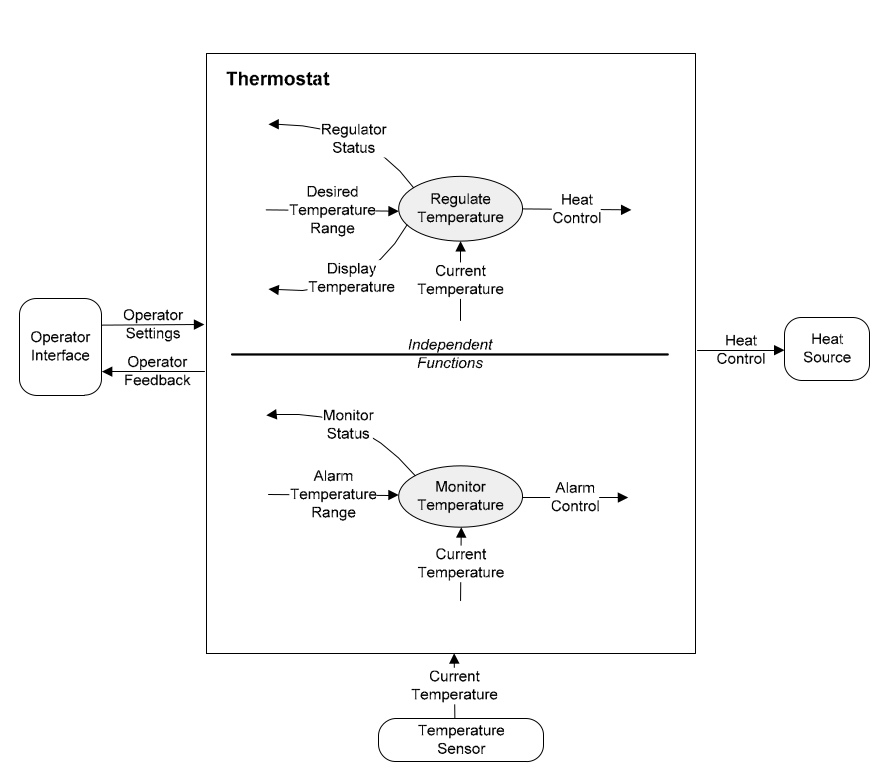
\includegraphics[width=\textwidth]{figures/thermostat-dependency-diagram.png}}
  \vspace{-.4cm}
  \caption{Thermostat Dependency Diagram}
  \vspace{-.4cm}
 \label{fig:dependency}
\end{figure*}

\section{Regulate Temperature Function}
\label{sec:regulate-temperature-function}

The Regulate Temperature Function compares the Current Temperature from the Temperature
Sensor with the Desired Temperature Range provided by the Operator Interface and turns the
Heat Source on or off to keep the Current Temperature within the Desired Temperature Range.
It also provides the Display Temperature and the Regulator Status back to the Operator Interface.

The high-level requirements for the Regulate Temperature Function are as follows:

\begin{itemize}
\item REQ-RT-1: The Regulate Temperature Function shall set the value of the Heat Control.

      Rationale: The primary function of the Regulate Temperature Function is to turn the
      Heat Control on and off to maintain the Current Temperature in the Isolette within the
      Desired Temperature Range, as required by SR-1.
\item REQ-RT-2: The Regulate Temperature Function shall set the value of the Regulator
      Status.

      Rationale: The status of the Regulate Temperature Function is provided to the Operator
      Interface so it can use the status of the Regulate Temperature and Monitor Temperature
      Functions to report the overall status of the Thermostat, as required by SR-1.
\item REQ-RT-3: The Regulate Temperature Function shall set the value of the Display
      Temperature.

      Rationale: The Current Temperature of the Isolette is displayed on the Operator Interface
      to provide the operators with an additional means to confirm that the Isolette is
      maintaining the temperature correctly. This value is provided by the Regulate
      Temperature Function to the Operator Interface as the Display Temperature.
\end{itemize}

The Regulate Temperature Function is allocated into subfunctions in figure ~\ref{fig:temp-dependency}.

\begin{figure*}[ht]
  \centerline{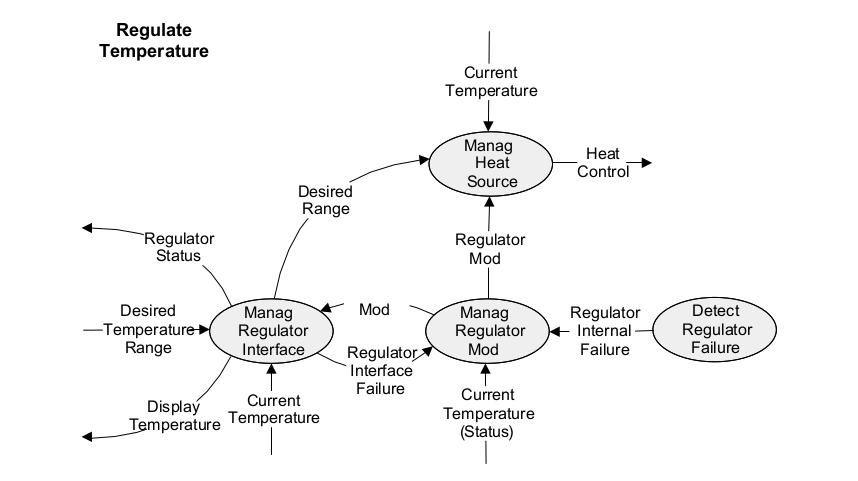
\includegraphics[width=\textwidth]{figures/regulate-temperature-dependency.png}}
  \vspace{-.4cm}
  \caption{Regulate Temperature Dependency Diagram}
  \vspace{-.4cm}
 \label{fig:temp-dependency}
\end{figure*}

The internal variables for the Regulate Temperature Function are shown in table ~\ref{tab:internal-variables}.

\begin{table}
\begin{tabular}{|l|l|l|l|l|}
\hline
Name & Type & Range & Units & Physical Interpretation \\\hline
Desired Temperature &  &  &  & Desired range of Isolette temperature \\\hline
Lower Desired Temperature & Integer & [96..101] & °F & Lower value of desired range \\\hline
Upper Desired Temperature & Integer & [97..102] & °F & Upper value of desired range \\\hline
Regulator Interface Failure & Boolean & False, True &  & Indicates an operator interface \\\hline
Regulator Internal Failure & Boolean & False, True &  & Indicates an internal failure \\\hline
Regulator Mode & Enumerated & Init &  & Initializing following power-up \\\cline{3-5}
  &  & NORMAL &  & Normal mode of operation \\\cline{3-5}
  &  & FAILED &  & Internal failure detected \\\hline
\end{tabular}
\caption{The Regulate Temperature Internal Variables}
\label{tab:internal-variables}
\end{table}

\subsection{Manage Regulator Interface Function}
\label{subsec:MRI-fun}

The Manage Regulator Interface Function defines the interaction with the Operator Interface
external entity. These include obtaining the Desired Range, reporting back the status of the
Regulate Temperature Function, and reporting back the Display Temperature. The constants are
shown in table ~\ref{tab:MRI-fun-constants}.

\begin{table}
\begin{tabular}{|l|l|l|l|l|}
\hline
Name & Type & Range & Units & Physical Interpretation \\\hline
Max Operator & Real & 0.5 & Sec & This time an operation will tolerate between an operator \\
Response Time &  &  &  & request or a change in the Thermostat state and the \\
  &  &  &  & visible response \\\hline
\multicolumn{5}{|l|}{Rationale: A trade study has shown that this lag should be no more than 0.5 second.} \\\hline
\end{tabular}
\caption{Manage Regulator Interface Function Constants}
\label{tab:MRI-fun-constants}
\end{table}

The requirements for the Regulator Status controlled variable are as follows:

\begin{itemize}
\item REQ-MRI-1: If the Regulator Mode is INIT, the Regulator Status shall be set to Init.
\item REQ-MRI-2: If the Regulator Mode is NORMAL, the Regulator Status shall be set to On.
\item REQ-MRI-3: If the Regulator Mode is FAILED, the Regulator Status shall be set to Failed.

      Latency: $<$ Max Operator Response Time
      Tolerance: N/A
\end{itemize}

The requirements for the Display Temperature controlled variable are as follows:

\begin{itemize}
\item REQ-MRI-4: If the Regulator Mode is NORMAL, the Display Temperature shall be set
      to the value of the Current Temperature rounded to the nearest integer.

      Rationale: Displaying the rounded value of the Current Temperature provides the the
      most accurate display of the Current Temperature possible using an integer display.
      When combined with the accuracy of the Temperature Sensor (EA-TS-2), the Display
      Temperature should be within 0.6°F of the actual value.
\item REQ-MRI-5: If the Regulator Mode is not NORMAL, the value of the Display Temperature is UNSPECIFIED.

      Rationale: In modes other than NORMAL, the value of Display Temperature is not
      meaningful and should not be used.

      Latency: $<$ Max Operator Response Time

      Tolerance: ±0.6°F
\end{itemize}

The requirements for the Regulator Interface Failure internal variable are as follows:

\begin{itemize}
\item REQ-MRI-6: If the Status attribute of the Lower Desired Temperature or the Upper
      Desired Temperature is Invalid, the Regulator Interface Failure shall be set to True.
\item REQ-MRI-7: If the Status attribute of the Lower Desired Temperature and the Upper
      Desired Temperature is Valid, the Regulator Interface Failure shall be set to False.

      Rationale: The Regulator Interface Failure internal variable indicates if any errors have
      occurred in sensing the Operator Interface monitored variables needed by the Regulate
      Temperature Function. Note that its initial value on power-up will always be True since
      the Status of the Lower Desired Temperature and the Upper Desired Temperature are
      initially Invalid.
\end{itemize}

The requirements for the Desired Range internal variable are as follows:

\begin{itemize}
\item REQ-MRI-8: If the Regulator Interface Failure is False, the Desired Range shall be set to
      the Desired Temperature Range.
\item REQ-MRI-9: If the Regulator Interface Failure is True, the Desired Range is UNSPECIFIED.

      Rationale: The Desired Range is only meaningful when there is not a Regulator Interface
      Failure. If there is, its value should not be used, and it can be set to any value.
\end{itemize}

\subsection{Manage Regulator Mode Function}
\label{subsec:MRM-fun}

The Manage Regulator Mode Function determines the mode of the Regulate Temperature
Function. The constants and definitions are shown in tables ~\ref{tab:MRM-fun-constants} and ~\ref{tab:MRM-fun-definitions}, respectively.

\begin{table}
\begin{tabular}{|l|l|l|l|l|}
\hline
Name & Type & Range & Units & Physical Interpretation \\\hline
Regulator & Real & 1.0 & Sec & The time allowed for initialization of the Regulate \\
Init Timeout &  &  &  & Temperature Function before declaring failure \\\hline
\multicolumn{5}{|l|}{Rationale: A trade study has shown that users become impatient if the Thermostat requires} \\
\multicolumn{5}{|l|}{more than one second to initialize.} \\\hline
\end{tabular}
\caption{The Manage Regulator Mode Function Constants}
\label{tab:MRM-fun-constants}
\end{table}

\begin{table}
\begin{tabular}{|l|l|l|}
\hline
Name & Type & Definition \\\hline
Regulator Status & Boolean & NOT (Regulator Interface Failure OR Regulator Internal Failure) \\
  &  & AND Current Temperature.Status = Valid \\\hline
\end{tabular}
\caption{The Manage Regulator Mode Function Definitions}
\label{tab:MRM-fun-definitions}
\end{table}

The requirements for the Regulator Mode internal variable are as follows:

\begin{itemize}
\item The modes and transitions of the Manage Regulator Mode Function are specified in the
      state transition diagram shown in figure ~\ref{fig:RTMT-diagram}. Each transition is a separate requirement
      and is assigned a unique identifier (e.g., Req MRM 1). All transitions are assumed to
      occur in negligible time.

      Rationale: (Req MRM 3 and Req MRM 4) Once the regulator has failed, the only way
      for it to re-enter normal operation is for it to be powered off and on. This ensures that the
      operators are made aware of any transient failures that the regulator may be experiencing.
\end{itemize}

\begin{figure*}[ht]
  \centerline{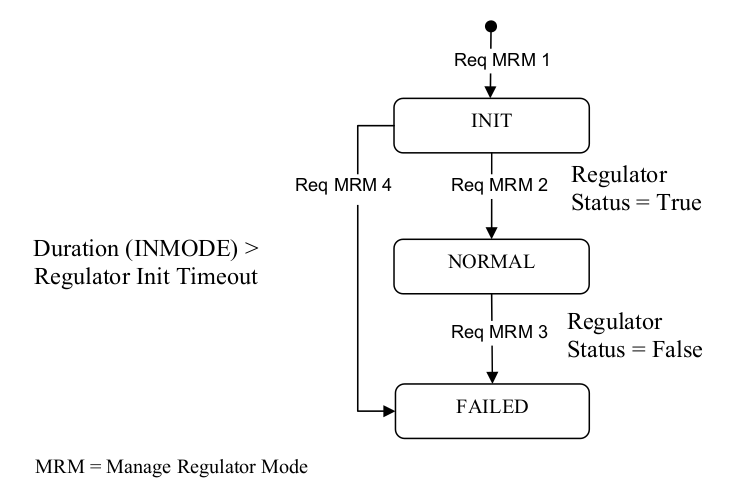
\includegraphics[width=\textwidth]{figures/regulate-temperature-mode-transition.png}}
  \vspace{-.4cm}
  \caption{Regulate Temperature Mode Transition Diagram}
  \vspace{-.4cm}
 \label{fig:RTMT-diagram}
\end{figure*}

\subsection{Manage Heat Source Function}
\label{subsec:manage-heat-source}

The Manage Heat Source Function turns the Heat Source on and off to maintain the Current
Temperature of the Isolette within the Desired Temperature Range. The constants are shown in
table ~\ref{tab:MHSF-constants}.

\begin{table}
\begin{tabular}{|l|l|l|l|l|}
\hline
Name & Type & Range & Units & Physical Interpretation \\\hline
Allowed Heat & Real & 6.0 & Sec & The maximum time by which the Heat Source \\
Source Latency &  &  &  & must be turned on or off to ensure acceptable  \\
  &  &  &  & Operation of the Isolette system \\\hline
\multicolumn{5}{|l|}{Since a closed Isolette will warm or cool at a maximum rate of 1°F per minute} \\
\multicolumn{5}{|l|}{(EA-IS1 and EA-IS2), turning the Heat Source on or off within 6 seconds ensures that the} \\
\multicolumn{5}{|l|}{Current Temperature will not have changed by more than 0.1°F, the required accuracy and} \\
\multicolumn{5}{|l|}{resolution of the Temperature Sensor (EA-TS2).} \\\hline
\end{tabular}
\caption{The Manage Heat Source Function Constants}
\label{tab:MHSF-constants}
\end{table}

The requirements for the Heat Control controlled variable are as follows:

\begin{itemize}
\item REQ-MHS-1: If the Regulator Mode is INIT, the Heat Control shall be set to Off.

      Rationale: A regulator that is initializing cannot regulate the Current Temperature of the
      Isolette and the Heat Control should be turned off.
\item REQ-MHS-2: If the Regulator Mode is NORMAL and the Current Temperature is less
      than the Lower Desired Temperature, the Heat Control shall be set to On.
\item REQ-MHS-3: If the Regulator Mode is NORMAL and the Current Temperature is
      greater than the Upper Desired Temperature, the Heat Control shall be set to Off.
\item REQ-MHS-4: If the Regulator Mode is NORMAL and the Current Temperature is
      greater than or equal to the Lower Desired Temperature and less than or equal to the
      Upper Desired Temperature, the value of the Heat Control shall not be changed.

      Rationale: When the Isolette is warming towards the Upper Desired Temperature, the
      Heat Source should be left on until the Upper Desired Temperature is reached. In a
      similar fashion, if the Isolette is cooling towards the Lower Desired Temperature, the
      Heat Source should be left off until the Lower Desired Temperature is reached.
\item REQ-MHS-5: If the Regulator Mode is FAILED, the Heat Control shall be set to Off.

      Rationale: In failed mode, the regulator cannot regulate the Current Temperature of the
      Isolette and the Heat Control should be turned off.

      Latency: $<$ Allowed Heat Source Latency

      Tolerance: N/A
\end{itemize}

\subsection{Detect Regulator Failure Function}
\label{subsec:detect-regulator-failure}

The Detect Regulator Failure Function identifies internal failures, (e.g., a memory check failure)
in the Regulate Temperature Function. It defines a single Boolean-valued internal variable,
Regulator Internal Failure, which is set to True if an internal failure is detected.

The requirements for Regulator Internal Failure variable are implementation-specific and cannot
be specified until an implementation platform is chosen.

\section{Monitor Temperature Function}
\label{sec:monitor-temperature}

The Monitor Temperature Function compares the Current Temperature from the Temperature
Sensor with the Alarm Temperature Range provided by the Operator Interface and turns the
Alarm Control on or off to Alert The Nurse if the Current Temperature falls below or rises above
the safe range. It also provides the Monitor Status back to the Operator Interface.

The high-level requirements for the Monitor Temperature Function are as follows:

\begin{itemize}
\item REQ-MT-1: The Monitor Temperature Function shall set the value of the Alarm Control.

      Rationale: The primary function of the Monitor Temperature Function is to raise an
      alarm if the Isolette is unable to maintain the Current Temperature within the Alarm
      Temperature Range, as required by safety requirement SR-2.
\item REQ-MT-2: The Monitor Temperature Function shall set the value of the Monitor Status.

      Rationale: Safety requirement SR-2 requires the Thermostat to provide an independent
      monitor function. The status of this function must be provided to the Operator Interface,
      which will use it and the status of the Regulate Temperature Function to report the
      overall status of the Thermostat, as required by safety requirement SR-2.
\end{itemize}

The Monitor Temperature Function is allocated into subfunctions as shown in figure ~\ref{fig:monitor-temp-dependency}.

\begin{figure*}[ht]
  \centerline{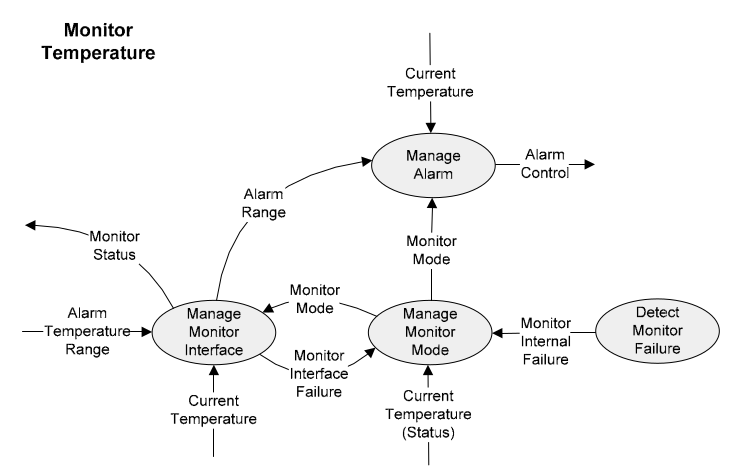
\includegraphics[width=\textwidth]{figures/monitor-temperature-dependency.png}}
  \vspace{-.4cm}
  \caption{Monitor Temperature Dependency Diagram}
  \vspace{-.4cm}
 \label{fig:monitor-temp-dependency}
\end{figure*}

The Monitor Temperature internal variables are shown in table ~\ref{tab:MTI-variables}.

\begin{table}
\begin{tabular}{|l|l|l|l|l|}
\hline
Name & Type & Range & Units & Physical Interpretation \\\hline
Alarm Range &  &  &  & Safe range of Isolette temperature \\\hline
Lower Alarm Temperature & Integer & [96..101] & °F & Lower value of alarm range \\\hline
Upper Alarm Temperature & Integer & [97..102] & °F & Upper value of alarm range \\\hline
Monitor Interface Failure & Boolean & False, True &  & Indicates an operator interface failure \\\hline
Monitor Internal Failure & Boolean & False, True &  & Indicates an internal failure \\\hline
Monitor Mode & Enumerated & Init &  & Initializing following power-up \\\cline{3-5}
  &  & NORMAL &  & Normal mode of operation \\\cline{3-5}
  &  & FAILED &  & Internal failure detected \\\hline
\end{tabular}
\caption{Monitor Temperature Internal Variables}
\label{tab:MTI-variables}
\end{table}

\subsection{Manage Monitor Interface Function}
\label{subsec:MMIF}

The Manage Monitor Interface function defines the interaction with the Operator Interface
external entity. These include obtaining the Alarm Range and reporting back the status of the
Monitor Temperature Function. The constants are shown in table ~\ref{tab:MMIF-constants}.

\begin{table}
\begin{tabular}{|l|l|l|l|l|}
\hline
Name & Type & Range & Units & Physical Interpretation \\\hline
Max Operator & Real & 0.5 & Sec & This time an operation will tolerate between an operator \\
Response Time &  &  &  & request or a change in the Thermostat state and the \\
  &  &  &  & visible response \\\hline
\multicolumn{5}{|l|}{Rationale: A trade study has shown that this lag should be no more than 0.5 second.} \\\hline
\end{tabular}
\caption{The Manage Monitor Interface Function Constants}
\label{tab:MMIF-constants}
\end{table}

The requirements for the Monitor Status controlled variable are as follows:

\begin{itemize}
\item REQ-MMI-1: If the Manage Monitor Interface mode is INIT, the Monitor Status shall be
      set to Init.
\item REQ-MMI-2: If the Manage Monitor Interface mode is NORMAL, the Monitor Status
      shall be set to On.
\item REQ-MMI-3: If the Manage Monitor Interface mode is FAILED, the Monitor Status
      shall be set to Failed.

      Latency: $<$ Max Operator Response Time

      Tolerance: N/A
\end{itemize}

The requirements for Monitor Interface Failure internal variable are as follows:

\begin{itemize}

\item REQ-MMI-4: If the Status attribute of the Lower Alarm Temperature or the Upper
      Alarm Temperature is Invalid, the Monitor Interface Failure shall be set to True.
\item REQ-MMI-5: If the Status attribute of the Lower Alarm Temperature and the Upper
      Alarm Temperature is Valid, the Monitor Interface Failure shall be set to False.

      Rationale: The Monitor Interface Failure internal variable indicates if any errors have
      occurred in sensing the Operator Interface monitored variables needed by the Manage
      Temperature Function. Note that its initial value on power-up will always be True since
      the Status attribute of the Lower Alarm Temperature and the Upper Alarm Temperature
      will initially be Invalid.
\end{itemize}

The requirements for Alarm Range Internal variable are as follows:

\begin{itemize}
\item REQ-MMI-6: If the Monitor Interface Failure is False, the Alarm Range variable shall
      be set to the Desired Temperature Range.
\item REQ-MMI-7: If the Monitor Interface Failure is True, the Alarm Range variable is
      UNSPECIFIED.

      Rationale: The Alarm Range variable is only meaningful when there is not a Monitor
      Interface Failure. If there is, its value should not used and it can be set to any value.
\end{itemize}

\subsection{Manage Monitor Mode Function}
\label{subsec:MMMF}

The Manage Monitor Mode Function determines the mode of the Monitor Temperature
Function. The constants and definitions are shown in tables ~\ref{tab:MMMF-constants} and ~\ref{tab:MMMF-definitions}, respectively.

\begin{table}
\begin{tabular}{|l|l|l|l|l|}
\hline
Name & Type & Range & Units & Physical Interpretation \\\hline
Monitor & Real & 1.0 & Sec & The time allowed for initialization of the Monitor \\
Initialization &  &  &  & Temperature Function before declaring failure \\
Timeout &  &  &  &  \\\hline
\multicolumn{5}{|l|}{Rationale: A trade study has shown that users become impatient if the Thermostat requires} \\
\multicolumn{5}{|l|}{more than one second to initialize.} \\\hline
\end{tabular}
\caption{The Manage Monitor Mode Function Constants}
\label{tab:MMMF-constants}
\end{table}

\begin{table}
\begin{tabular}{|l|l|l|}
\hline
Name & Type & Definition \\\hline
Monitor Status & Boolean & NOT (Monitor Interface Failure OR Monitor Internal Failure) \\
  &  & AND Current Temperature.Status = Valid \\\hline
\end{tabular}
\caption{The Manage Monitor Mode Function Definitions}
\label{tab:MMMF-definitions}
\end{table}

The requirements for the Regulator Mode internal variable are as follows:

\begin{itemize}
\item The modes and transitions of the Manage Regulator Mode Function are specified in the
      state transition diagram shown in figure ~\ref{fig:MTMT}. Each transition is a separate requirement
      and is assigned a unique identifier (e.g., Req MRM 1). All transitions are assumed to
      occur in negligible time.

      Rationale: (Req MRM 3 and Req MRM 4) Once the regulator has failed, the only way
      for it to re-enter normal operation is for it to be powered off and on. This ensures that the
      operators are made aware of any transient failures that the regulator may be experiencing.
\end{itemize}

\begin{figure*}[ht]
  \centerline{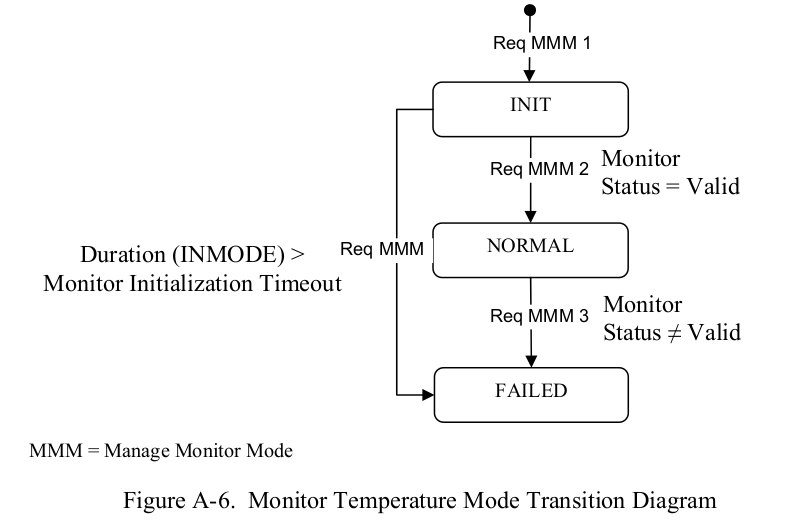
\includegraphics[width=\textwidth]{figures/monitor-temperature-mode-transition.png}}
  \vspace{-.4cm}
  \caption{Monitor Temperature Mode Transition Diagram}
  \vspace{-.4cm}
 \label{fig:MTMT}
\end{figure*}

\subsection{Manage Alarm Function}
\label{subsec:manage-alarm-function}

The Manage Alarm Function turns the Alarm Control on when the Current Temperature of the
Isolette falls below or rises above the Alarm Temperature Range.

The requirements for the Alarm Control controlled variable are as follows:

\begin{itemize}
\item REQ-MA-1: If the Monitor Mode is INIT, the Alarm Control shall be set to Off.

      Rationale: A monitor that is initializing should not activate the alarm unless it enters the
      FAILED mode.
\item REQ-MA-2: If the Monitor Mode is NORMAL and the Current Temperature is less than
      the Lower Alarm Temperature or greater than the Upper Alarm Temperature, the Alarm
      Control shall be set to On.
\item REQ-MA-3: If the Monitor Mode is NORMAL and the Current Temperature is greater
      than or equal to the Lower Alarm Temperature and less than the Lower Alarm
      Temperature +0.5°, or the Current Temperature is greater than the Upper Alarm
      Temperature -0.5° and less than or equal to the Upper Alarm Temperature, the value of
      the Alarm Control shall not be changed.

      Rationale: This provides a hysteresis that prevents transient alarms, see figure ~\ref{fig:alarm-hyperesis}.
\item REQ-MA-4: If the Monitor Mode is NORMAL and the value of the Current
      Temperature is greater than or equal to the Lower Alarm Temperature +0.5° and less than
      or equal to the Upper Alarm Temperature -0.5°, the Alarm Control shall be set to Off.

      Rationale: This turns the alarm off at the same moment that the Displayed Temperature
      shows a value greater than the Lower Alarm Temperature and less than the Upper Alarm
      Temperature.
\item REQ-MA-5: If the Monitor Mode is FAILED, the Alarm Control shall be set to On.

      Rationale: A failed monitor cannot monitor the Current Temperature of the Isolette and
      the Alarm should be turned on.

      Latency: $<$5 seconds

      Tolerance: N/A

      Rationale: Required by SR-2.
\end{itemize}

\begin{figure*}[ht]
  \centerline{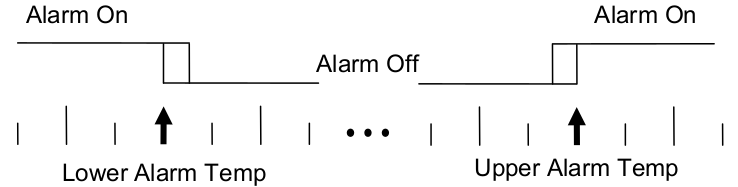
\includegraphics[width=\textwidth]{figures/transient-alarm-hysteresis.png}}
  \vspace{-.4cm}
  \caption{Transient Alarm Hyperesis}
  \vspace{-.4cm}
 \label{fig:alarm-hyperesis}
\end{figure*}

\subsection{Detect Monitor Failure Function}
\label{subsec:DMFF}

The Detect Monitor Failure Function identifies internal failures, (e.g., a memory check failure)
in the Monitor Temperature Function. It defines a single Boolean-valued internal variable,
Monitor Internal Failure, which is set to True if an internal failure is detected.

The requirements for Monitor Internal Failure variable are implementation-specific and cannot
be specified until an implementation platform is chosen.

\end{document}